\section{NAX通证经济设计}
\subsection{设计目标}
设计公链的通证经济的目标除了更好的激活生态外,而且需要在公链生态中起到积极正向的作用。公链的通证经济的核心设计应当符合一定的原则和目标,例如:公平受益、正向激励、逻辑简洁,场景多样等。总而言之,公链的通证经济需要公正的获取场景和多样的消耗场景,使得通证拥有更高的持有价值,从而促进公链的发展和壮大,一个良好的公链通证经济,会使得整个生态变得更加有活力和动力。总结起来NAX的设计目标是:

\begin{enumerate}[\hspace{2cm}(a)]
    \item 公平受益
    \item 正向激励
    \item 简洁易懂
    \item 场景丰富
    \item 智能有效
\end{enumerate}

\subsection{核心逻辑}

\subsubsection{资产公平性与正当性}
公链通证经济的有效性的根本来自于资产获得的公平性和正当性。资产的获取规则应当简单透明,对绝大多数人应当是信息对称的。在公链的通证经济中,公链的资产的所有权,具体比较公认的公平性,因此通过质押(Staking)的方法作为获取通证权益的主要途径是符合要求的。不会因为规则不清晰,或者漏洞导致错配现象,而且更多的变量根植说规则清晰后的博弈当中,并使得博弈的总体结果是有利于公链生态发展的方法。在星云的生态当中,质押(Staking)NAS,通过锁住NAS的流动性,以获取相应的NAX权益,这在星云生态通证经济体内是公平公正的。

\subsubsection{星云式智能质押}
传统的质押方式是用户将资产转入到智能合约当中暂为保管,使得大量的资产安全问题维系在一个智能合约里,这种中心化的质押,不禁让大家想法2016年以太坊的The DAO攻击事件,攻击者利用了合约漏洞使得投资者产生巨大的经济损失,也使得投资者对合约安全性产生怀疑。另一方面,质押同时也给公链项目方带来非常大的压力,大量资产保存在一个合约当中,使得合约的管理和安全性成为非常一个发展瓶颈。区块链上的资产是确权的,质押(Staking)只是锁住流动性,并不是资产的确权性(虽然可以通过调用合约方法取回)转移到合约里。

通过设计NAX的机制,我们提出星云式质押(Nebulas Smart Staking),在确保用户资的确权仍然属于用户的前提下,用户与质押合约签定的锁住流动性的契约记录在合约上。质押合约的作用只是通过随机链上检查契约的有效性来保持用户的质押有效性。星云式智能质押的优点是:
\begin{enumerate}[\hspace{2cm}(a)]
    \item 保证用户的资产确权
    \item 激励更多的用户参与质押
    \item 资产安全性去中心化
    \item 资产的确权性与锁住资产流动性分离
\end{enumerate}

\subsubsection{NAX增发模式 - IDO}
如上述提到的,在保障资产公平性与正当性基础上,确保用户质押资产所有权神圣不可侵犯的前提下,用户贡献出资产的流动性以获取相应的生态权益。我们称这种新式增发模式为IDO(Initial Devotion Offering)。NAX的预计发行总量上限是1,000亿(10 10)。 增发周期为每6,000高度(一天左右),每周期增发数量呈递减规律,衰减系数$\mu=0.999$,预计12年左右发放完全。

\subsubsection{NAX滚动分发模式}
NAX的每个周期$i$, 系统会预增发 $C_i$ 个NAX用来分配给目前正在质押的用户,系统在实际分布的时候会参考当前的质押率水平 r(当前参与质押NAS的总量/总体NAS流通总量)实际分发 $C_i$ * $\lambda_i$ (0<$\lambda_i$<1)个NAX,剩余未分发的 $C_i$ * (1 - $\lambda$) NAX将滚动到下一个周期的预增发总量里。其中,分发系数\(\lambda_i\)与质押率\(r_i\)的函数关系如以下公式所示,其函数关系如图\ref{func}所示。

  \begin{equation}
    \lambda_i = l r_i^3 + m r_i^2 + n r_i
  \end{equation}

\begin{figure}
\centering
    \begin{tikzpicture}
    \begin{axis}[
        axis lines = left,
        xlabel = {质押率$x_i$},
        ylabel = {发放比率$\lambda_i$},
    ]
    \addplot [
        domain=0:1,
        samples=100,
        color=blue,
    ]
    {1.52*x^3-3.88*x^2+3.36*x};
    \addplot [
        domain=-0:1, 
        samples=100, 
        color=red,
    ]
    {1};
    \end{axis}
    \end{tikzpicture}
    \caption{增发比例与质押率的关系}\label{func}
\end{figure}




NAX的核心系统将以每6,000高度(一天左右)作为一个增发周期。每个周期将根据有一个固定的待增发量,当去的质押比率情况进行不同程度的增发。每周期过后,增发参数将以一程度衰减。一个直观的效果,经过一年之后,增发系数将会衰减到初始的一半左右。

公式如下:

\begin{equation}
  K_{i,j} = \frac{P_{i,j} f(T_{i,j})}{\sum_j P_{i,j} f(T_{i,j})} \lambda_i C_i
\end{equation}

其中,
\begin{enumerate}
   \item \(K_{i,j}\): 第\(i\)期用户\(j\)获得的Token数量
   \item \(P_{i,j}\): 第\(i\)期用户\(j\)的质押量
   \item \(f(T_{i,j})\): 第\(i\)期用户\(j\)的质押的有效权重
   \item \(T_{i,j}\): 第\(i\)期用户\(j\)的累积质押周期数(从质押时开始计算)
   \item \(\lambda_i\): 第\(i\)期增发比例
   \item \(C_i\): 第\(i\)期增发池,\(C_i = C_0 \mu^i + C_{i-1} (1-\lambda_{i-1})\),包含两部分。第一部分为基础部分,每一期不断衰减,衰减系数$\mu=0.9981$。第二部分为上一期增发池中的剩余部分。
\end{enumerate}

质押的有效权重与质押周期数的函数\(f(T)\)的形式为
  \begin{equation}
    f(T) = 1 - \frac{\sqrt{(aT+b)^2+c^2}-(aT+b)}{2}
  \end{equation}
其中\(a=0.005\),\(b=-0.3\),\(c=0.2\),该函数如图\ref{weight}所示。可见有效权重的值在0.67到1之间,随质押周期数的增加而不断接近1,质押周期数为30(约1个月)时有效权重为0.8,质押周期数为60(约2个月)时有效权重为0.9,质押周期数为90(约3个月)时有效权重为0.95。

\begin{figure}
\centering
    \begin{tikzpicture}
    \begin{axis}[
        axis lines = left,
        xlabel = {质押周期数},
        ylabel = {有效权重},
    ]
    \addplot [
        domain=0:365,
        samples=200,
        color=blue,
    ]
    {1-(sqrt((0.005*x-0.3)^2+0.2^2)-(0.005*x-0.3))/2};

    \addplot [
        domain=-0:365, 
        samples=200, 
        color=red,
    ]
    {1};
    \end{axis}
    \end{tikzpicture}
    \caption{质押的有效权重与质押周期数的关系}\label{weight}
\end{figure}

增发比例\(\lambda_i\)与质押率\(x_i\)(总质押量与总流通量之比)相关,
增发比例与质押率的函数关系为
  \begin{equation}
    \lambda_i = l x_i^3 + m x_i^2 + n x_i
  \end{equation}
增发比例与质押率的关系如图\ref{func}所示。可见增发比例的取值在0到1之间,质押率为30\%时增发比例为70\%,质押率为50\%时增发比例为90\%。





\begin{figure}
\centering
    \begin{tikzpicture}
    \begin{axis}[
        axis lines = left,
        xlabel = {周期数},
        ylabel = {每日预发行NAX数量},
    ]
    \addplot [
        domain=-0:1200, 
        samples=100,
        color=red,
    ]
    {1.9*10^7*0.9981^x};

    \end{axis}
    \end{tikzpicture}
    \caption{每日预发行NAX数量与周期关系}\label{acc0}
\end{figure}

%累积增发NAX数量与周期关系
\begin{figure}
\centering
    \begin{tikzpicture}
    \begin{axis}[
        axis lines = left,
        xlabel = {周期数},
        ylabel = {累积预发行NAX数量},
    ]
    \addplot [
        domain=-0:2000, 
        samples=400, 
        color=red,
    ]
    {10^10*(1 - 0.9981^(x+1))};

    \addplot [
        domain=-0:2000, 
        samples=400, 
        color=blue,
    ]
    {10^10};
    \end{axis}
    \end{tikzpicture}
\caption{累积增发NAX数量与周期关系}\label{acc1}
\end{figure}


由于每期增发池中未发放的部分滚入下一期增发池中,因此总发行量为固定值
\begin{equation}
  \sum_{i,j} K_{i,j} = \sum_i C_0 \mu^i = \frac{C_0}{1-\mu}
\end{equation}
令此上界为100亿(\(10^{10}\)),可解出\(C_0 = 10^{10}(1-\mu) = 1.9\times10^7\)。


同一个周期内,系统会根据质押数量以及相应的质押时间长短来分配增发的总量,以达到公平的效果,即质押数量越多,质押时间越长,所分配到的增发数量也会更多。该设计会达到以下博弈场景:
\begin{enumerate}
  \item 早期参与质押的用户,有更大的概率获得更多的系统增发
  \item 随着质押率增加,系统增发数量也会相应提高,以鼓励更多人加入质押
\end{enumerate}

\subsection{合约框架}
NAX是由一组合约组成,是在NRC20基础上扩展的合约组,并配有多签合约管理整个合约里的参数,详细如图\ref{fig:nax_framework}所示。

\begin{figure}[htbp]
  \centering
    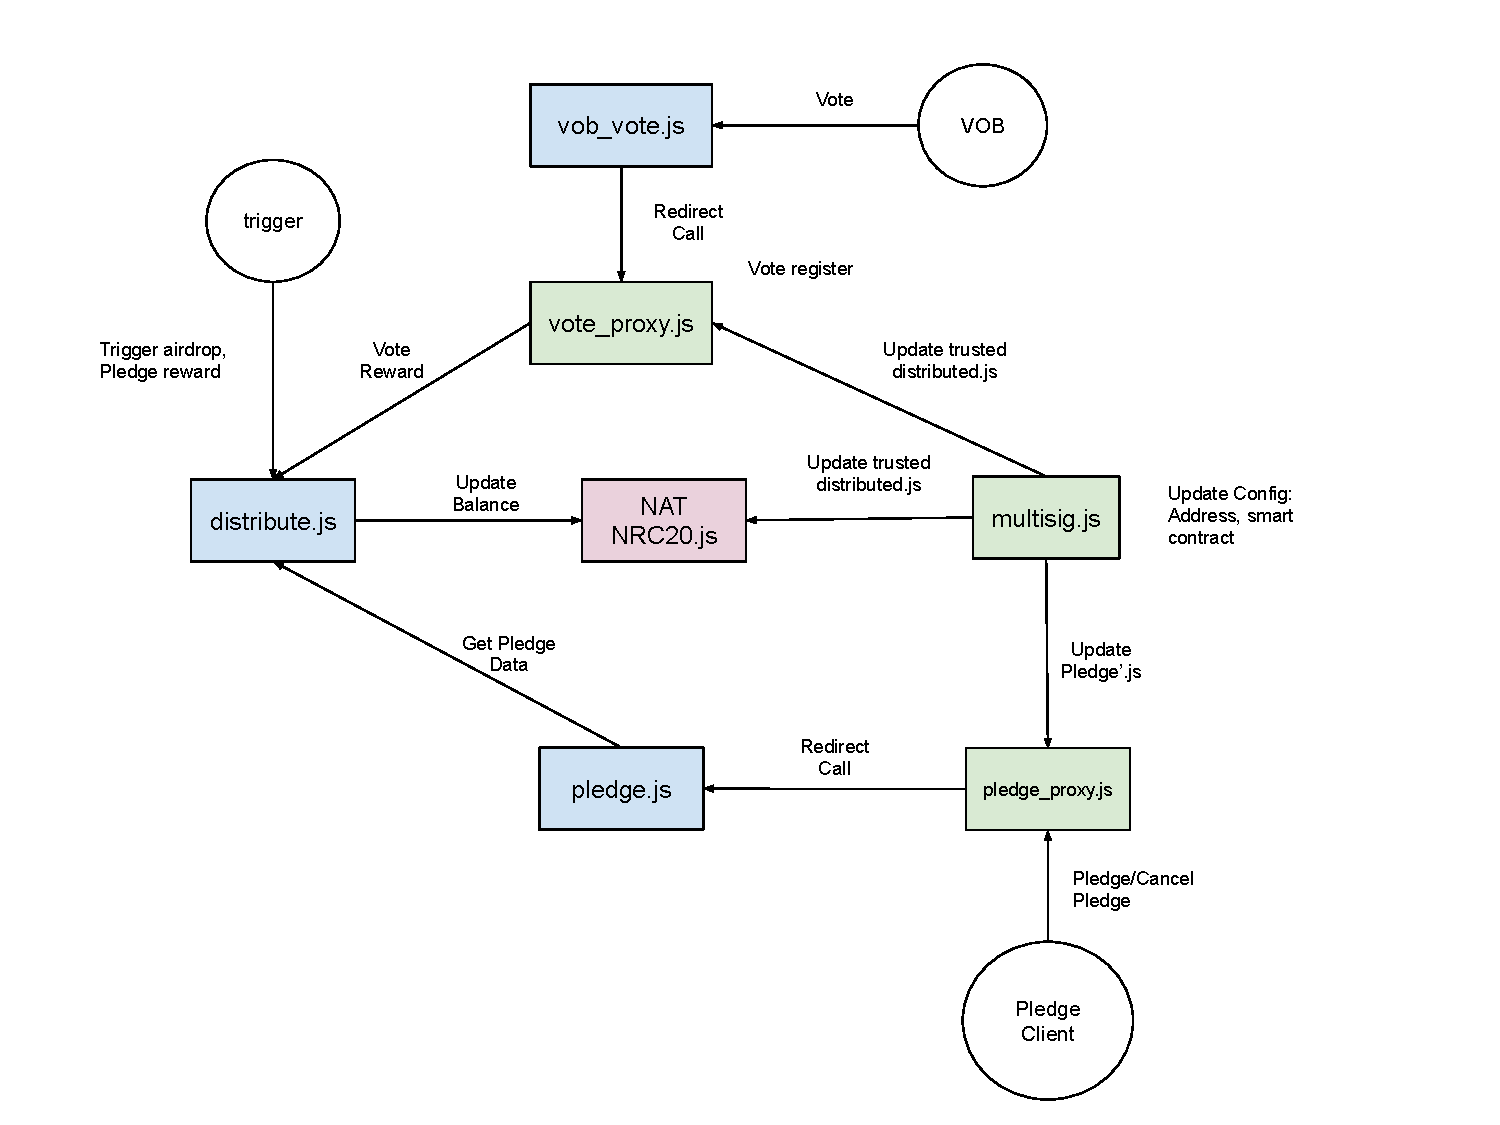
\includegraphics[width=1\textwidth]{../common/zh/nax.pdf}
    \caption{NAX 合约示意图(此图待更新) \label{fig:nax_framework}}
\end{figure}
